\documentclass{standalone}
%
\usepackage{tikz}
\usetikzlibrary{bending,arrows.meta}
\usepackage{tkz-euclide}
\usetkzobj{all}
\usepackage{xcolor}
%
\definecolor{earth}{HTML}{0089FA}
\definecolor{moon}{HTML}{AFAFAF}
%
\usepackage{fontspec}
\setmainfont{Open Dyslexic}
%
\title{Schema esperimenti di Michelson e Morley}
\begin{document}
	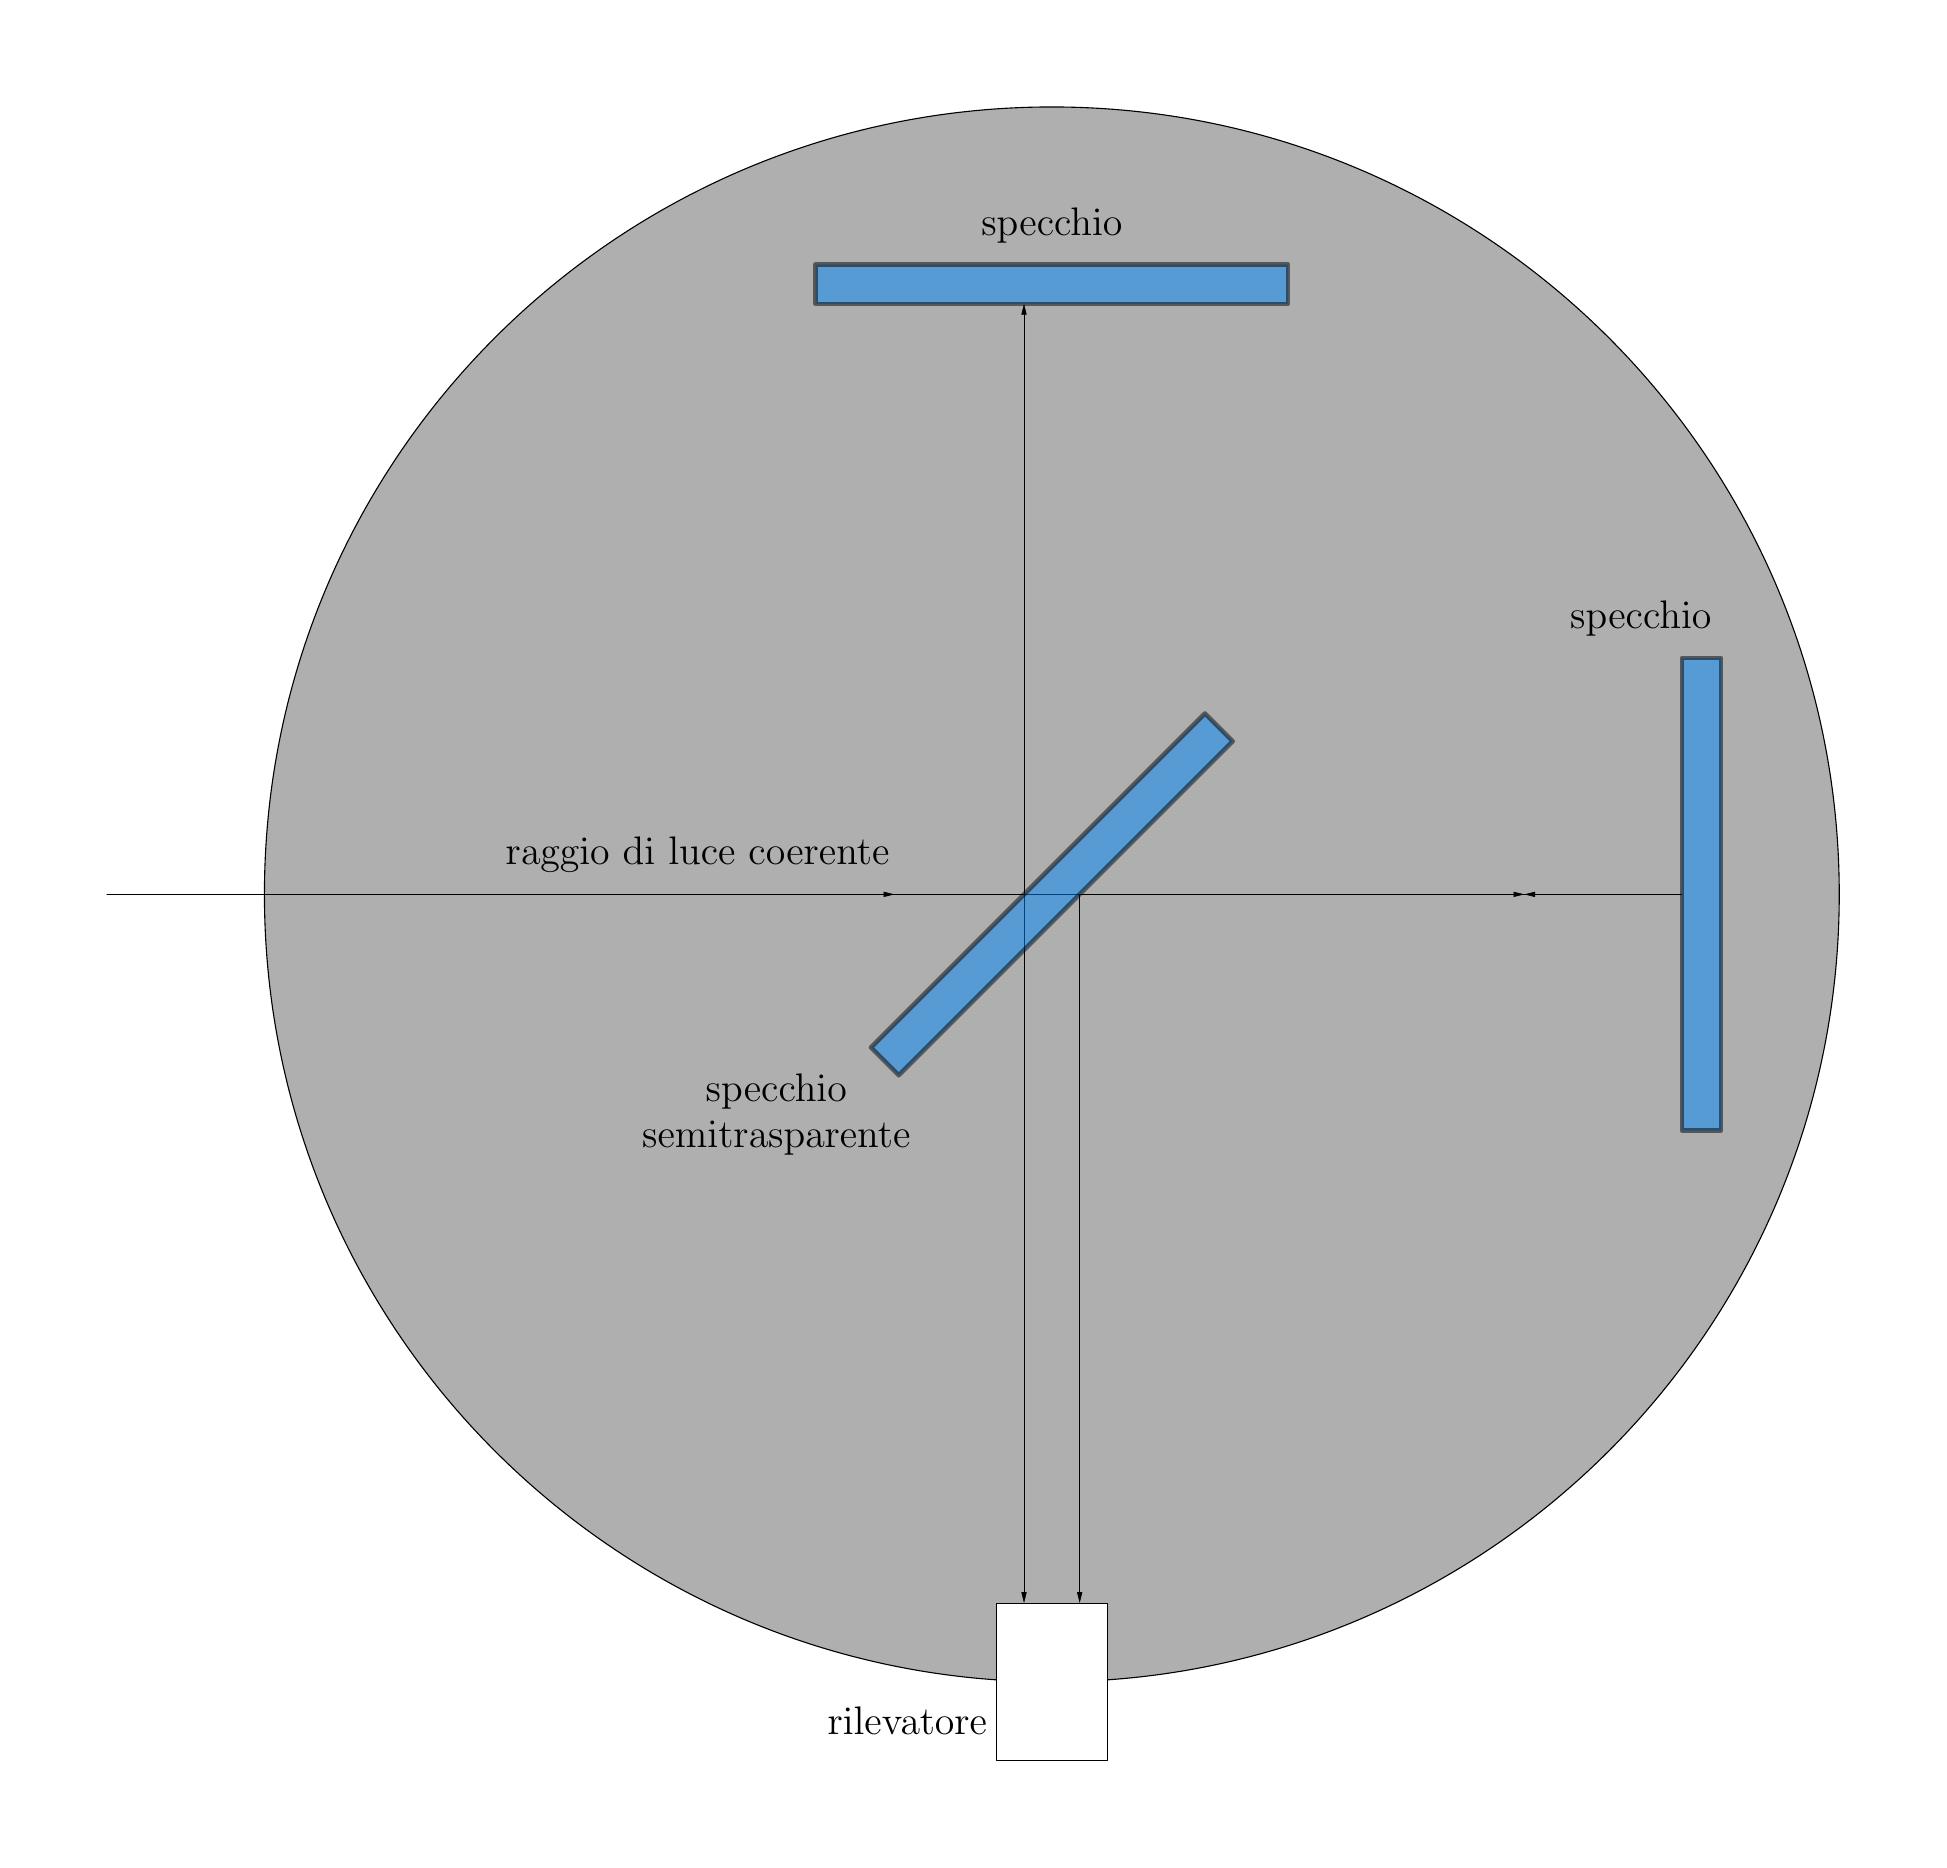
\begin{tikzpicture}[>={[inset=0,angle'=27]Stealth}]
		%
		\draw [use as bounding box,color=white] (-13,11) -| (-13,-12) |- (11,-12) -| (11,11);
		\begin{scope}
			\draw [fill=moon] (0,0) circle (10cm);
			%
			\tkzDefPoint(0,0){O}
			\tkzDefPoint(-3,0.25){A} \tkzDefPoint(3,0.25){B}
			\tkzDefPoint(3,-0.25){C} \tkzDefPoint(-3,-0.25){D}
			%
			\tkzDefPointBy[rotation = center O angle 45](A) \tkzGetPoint{A1}
			\tkzDefPointBy[rotation = center O angle 45](B) \tkzGetPoint{B1}
			\tkzDefPointBy[rotation = center O angle 45](C) \tkzGetPoint{C1}
			\tkzDefPointBy[rotation = center O angle 45](D) \tkzGetPoint{D1}
			%
			\tkzDefPoint(-12,0){R1} \tkzDefPoint(-2,0){F1}
			\tkzDefPoint(8,0){R2} \tkzDefPoint(6,0){F2}
			\tkzDrawSegment[->](R1,F1)
			\tkzDrawSegment[->](F1,F2)
			\tkzDrawSegment[<-](F2,R2)
			\tkzDrawSegment(R1,R2)
			%
			\tkzInterLL(R1,R2)(A1,B1) \tkzGetPoint{M1}
			\tkzDefLine[orthogonal=through M1](R1,R2) \tkzGetPoint{E}
			%
			\tkzDefPoint(-3,8){A2} \tkzDefPoint(3,8){B2}
			\tkzDefPoint(-3,7.5){D2} \tkzDefPoint(3,7.5){C2}
			\tkzInterLL(M1,E)(C2,D2) \tkzGetPoint{M2}
			\tkzDrawSegment[->](M1,M2)
			%
			\tkzDefPoint(8,-3){A3} \tkzDefPoint(8.5,-3){B3}
			\tkzDefPoint(8.5,3){C3} \tkzDefPoint(8,3){D3}
			%
			\tkzInterLL(R1,R2)(C1,D1) \tkzGetPoint{M3}
			\tkzDefLine[orthogonal=through M3](R2,R1) \tkzGetPoint{F1}
			\tkzDefLine[orthogonal=through M1](R2,R1) \tkzGetPoint{F2}
			%
			\tkzDefPoint(-0.7,-9){a} \tkzDefPoint(0.7,-9){b}
			\tkzDefPoint(0.7,-11){c} \tkzDefPoint(-0.7,-11){d}
			\tkzInterLL(M3,F1)(a,b) \tkzGetPoint{f1}
			\tkzDrawSegment[->](M3,f1)
			\tkzInterLL(M1,F2)(a,b) \tkzGetPoint{f2}
			\tkzDrawSegment[->](M1,f2)
			\tkzDrawPolygon[fill=white](a,b,c,d)
			%
			\tkzDrawPolygon[fill=earth,opacity=0.5,ultra thick](A1,B1,C1,D1)
			\tkzDrawPolygon[fill=earth,opacity=0.5,ultra thick](A2,B2,C2,D2)
			\tkzDrawPolygon[fill=earth,opacity=0.5,ultra thick](A3,B3,C3,D3)
			%
			\node at (0,8.5) {\textcolor{black}{\fontsize{15}{16}\selectfont specchio}};
			\node at (-4.5,0.5) {\textcolor{black}{\fontsize{15}{16}\selectfont raggio di luce coerente}};
			\node[left] at (8.5,3.5) {\textcolor{black}{\fontsize{15}{16}\selectfont specchio}};
			\node at (-3.5,-2.5) {\textcolor{black}{\fontsize{15}{16}\selectfont specchio}};
			\node at (-3.5,-3.1) {\textcolor{black}{\fontsize{15}{16}\selectfont semitrasparente}};
			\node[left] at (-0.7,-10.5) {\textcolor{black}{\fontsize{15}{16}\selectfont rilevatore}};
		\end{scope}
		%
	\end{tikzpicture}
\end{document}